\documentclass[11pt,a4paper]{article}
\usepackage[utf8]{inputenc}
\usepackage[T1]{fontenc}
\usepackage[spanish,es-noshorthands]{babel}
\usepackage{lmodern}
\usepackage[margin=2.5cm]{geometry}
\usepackage{booktabs}
\usepackage{tabularx}
\usepackage{enumitem}
\usepackage{graphicx}
\usepackage{float}
\usepackage{listings}
\usepackage{amsmath}
\usepackage[hidelinks]{hyperref}

\newcolumntype{Y}{>{\raggedright\arraybackslash}X}
\newcommand{\code}[1]{\texttt{#1}}
\graphicspath{{figuras/}}

\lstset{
  language=Python,
  basicstyle=\ttfamily\small,
  frame=single,
  columns=fullflexible,
  keepspaces=true,
  breaklines=true,
  showstringspaces=false,
  xleftmargin=4pt,
  xrightmargin=4pt,
}

\title{Motor de base de datos relacional en disco\\
\large Base de Datos II (CS2042)}
\author{Sebastian Hernandez Miñano \and David Huette Ospino \and
Luis Millones Carrasco \and Isaac Gamero del Aguila}
\date{23 de septiembre de 2026}

\begin{document}
\maketitle

\begin{center}
Repositorio: \url{https://github.com/Davidht77/proyecto-1-bd2}
\end{center}

\section{Resumen}

Construimos desde cero un gestor de bases de datos relacional que guarda todo en
disco, en páginas binarias de tamaño fijo. No usa ningún motor existente ni
librerías de serialización: cada byte se escribe con \code{struct} y cada página se
lee o escribe con un desplazamiento explícito dentro del archivo.

El sistema tiene seis capas:

\begin{enumerate}
  \item \textbf{Almacenamiento} (\code{backend/storage/}): páginas, archivos
        paginados y el contador de accesos a disco.
  \item \textbf{Organización de archivos} (\code{backend/structures/}): Heap File y
        Sequential File.
  \item \textbf{Índices} (\code{backend/index/}): Árbol B+ y Hashing Extensible.
  \item \textbf{Motor de consultas} (\code{backend/engine/}): parser SQL, catálogo,
        planificador y ejecutor.
  \item \textbf{API REST} (\code{backend/api/}): FastAPI.
  \item \textbf{Cliente web} (\code{frontend/}): React con cuatro paneles.
\end{enumerate}

Una regla atraviesa todo el diseño: \textbf{solo la capa de almacenamiento toca el
disco}. Si otro módulo abriera un archivo por su cuenta, el conteo de lecturas y
escrituras dejaría de ser exacto y los experimentos no valdrían nada.

\section{Capa de almacenamiento}

\subsection{Layout de página}

Todas las páginas del motor (datos, overflow, nodos del B+, buckets del hash)
comparten la misma cabecera de 32 bytes. Así, el lugar donde empiezan los datos se
calcula con una sola fórmula para todo el sistema.

\begin{lstlisting}
HEADER_SIZE = 32
# page_id(4) type(1) record_count(2) low_key_flag(1) free_space_offset(4)
# next(4) prev(4) aux(4) reserved(8) = 32 bytes
_HEADER = struct.Struct("<IBHBIIII8s")
\end{lstlisting}

\begin{itemize}
  \item \code{page\_id}: identificador del bloque dentro del archivo.
  \item \code{record\_count}: registros activos en la página.
  \item \code{free\_space\_offset}: inicio del espacio libre.
  \item \code{next} / \code{prev}: punteros para encadenar páginas. El Árbol B+ los
        usa como \code{next\_leaf\_id} y \code{prev\_leaf\_id}.
  \item \code{aux}: puntero de uso libre según la estructura (cabeza de la cadena de
        overflow, puntero $P_0$ del B+, profundidad local del bucket).
  \item \code{reserved}: 8 bytes que el Sequential File usa para guardar la clave
        mínima de la página (\code{low\_key}).
\end{itemize}

Elegimos \textbf{registros de longitud fija con bitmap de presencia}: cada slot tiene
un bit que dice si está ocupado. Como todos los tipos (\code{INT}, \code{FLOAT},
\code{CHAR(n)}) son de ancho fijo, el slot $i$ siempre está en el mismo offset, y la
búsqueda binaria dentro de una página es aritmética pura.

El bitmap y los registros compiten por el mismo espacio, así que la capacidad $C$ de
una página de tamaño $B$ con registros de $R$ bytes sale de resolver
$32 + \lceil C/8 \rceil + C \cdot R \le B$:

\begin{lstlisting}
def page_capacity(page_size, record_size):
    return (8 * (page_size - HEADER_SIZE)) // (8 * record_size + 1)
\end{lstlisting}

El \code{+1} del denominador es el bit del bitmap que cuesta cada slot. Con
$B = 4096$ y el registro de prueba de 32 bytes, caben 126 registros por página.

Cada tupla se identifica con un $\text{RID} = \langle \text{page\_id}, \text{slot}\rangle$.
El Sequential File agrega un tercer campo con el área (principal u overflow).

\subsection{Pager: el único que toca el disco}

La clase \code{Pager} administra un archivo paginado. Toda transferencia es de una
página completa y se hace con \code{os.pread}/\code{os.pwrite}, que reciben el
offset de forma explícita. En Windows se emula con \code{lseek} + \code{read}/\code{write}.

\begin{lstlisting}
def _pread(self, page_id):
    raw = _pread_at(self._fd, self.page_size, page_id * self.page_size)
    self.counter.record_read(self.page_size)
    return raw

def _pwrite(self, page_id, payload):
    _pwrite_at(self._fd, payload, page_id * self.page_size)
    self.counter.record_write(self.page_size)
\end{lstlisting}

La página física 0 de cada archivo es su cabecera: guarda el tamaño de página, el
número de páginas, la cabeza de la lista de páginas libres, el esquema de la tabla y
dos enteros de uso libre (\code{user\_a}, \code{user\_b}). Por eso los archivos son
\textbf{autodescriptivos}: el catálogo reconstruye todas las tablas leyendo solo la
página 0 de cada archivo, sin un archivo de catálogo aparte que se pueda
desincronizar.

Las páginas liberadas entran a una lista enlazada (\code{free\_page}); la siguiente
página que se pide reutiliza la primera de esa lista antes de agrandar el archivo.

\subsection{DiskCounter}

Un único \code{DiskCounter} se comparte entre todos los Pager de una tabla (datos,
overflow e índices), así que el desglose por consulta es total. Cuenta
\code{disk\_reads} y \code{disk\_writes} y ofrece un bloque \code{measure()} que
entrega las diferencias de una operación:

\begin{lstlisting}
with counter.measure() as m:
    tabla.search(101)
print(m.metrics.disk_reads, m.metrics.disk_writes, m.metrics.elapsed_ms)
\end{lstlisting}

\subsection{Buffer pool opcional}

Hay una caché LRU de escritura diferida (\code{buffer\_pool.py}), \textbf{apagada por
defecto}. Los experimentos corren sin caché para que cada \code{read\_page} sea una
transferencia física real y el conteo coincida con las fórmulas de costo. En la demo
se puede encender con \code{BD2\_CACHE\_SIZE}.

\section{Organización de archivos}

\subsection{Heap File}

Los registros se guardan sin orden. El archivo mantiene en su cabecera la cabeza de
una \textbf{free-list}: la página que todavía tiene espacio.

\begin{itemize}
  \item \textbf{Inserción, O(1) de I/O:} se lee la página de la free-list, se escribe
        el registro en su primer slot libre y se escribe la página. Si no hay página
        con espacio, se crea una al final.
  \item \textbf{Búsqueda:} recorrido completo de las $P$ páginas.
  \item \textbf{Eliminación con move-the-last:} el último registro del archivo se
        copia al hueco que deja el borrado. El archivo queda compacto sin huecos.
\end{itemize}

\begin{lstlisting}
last_record = last_page.read_record(last_slot)
del_page.write_record(rid.slot, last_record)
self._write_page(del_page)
last_page.set_occupied(last_slot, False)
last_page.record_count -= 1
self._write_page(last_page)
\end{lstlisting}

\subsection{Sequential File}

Usa dos archivos: \code{<tabla>.seq.dat} (área principal ordenada por la clave
primaria) y \code{<tabla>.seq.ovf} (área de overflow). La idea central es esta:

\begin{quote}
Los registros con clave en $[\text{low\_key}(p), \text{low\_key}(p+1))$ viven en la
página principal $p$ o en la cadena de overflow de $p$.
\end{quote}

\code{low\_key} es el rango \emph{declarado} de la página, no su primer registro.
Solo lo escriben la carga masiva y la reorganización. Si dependiera del primer
registro, al borrarlo el mínimo subiría y las claves menores que quedaran en overflow
se volverían inalcanzables.

\paragraph{Búsqueda binaria.} Se busca la última página cuyo \code{low\_key} es menor
o igual a la clave. La función devuelve también la página, para no releerla:

\begin{lstlisting}
lo, hi = 0, self.page_count - 1
while lo <= hi:
    mid = (lo + hi) // 2
    page = self._read_main(mid)
    if page.get_low_key(self.schema) <= key:
        resultado, pagina, lo = mid, page, mid + 1
    else:
        hi = mid - 1
\end{lstlisting}

Dentro de la página se hace otra búsqueda binaria sobre los slots. Si la clave no
está, se recorre la cadena de overflow de esa página, que también está ordenada, y se
corta en cuanto aparece una clave mayor.

\paragraph{Overflow.} Cada página principal tiene su propia cadena de páginas de
overflow (la cabeza vive en \code{aux}). Encadenamos \emph{páginas} y no registros
sueltos: en un sistema paginado, encadenar registro por registro costaría una lectura
por registro. Cuando una página de overflow se llena, se parte en dos mitades.

\paragraph{Cuándo reorganizar.} El área de overflow tiene un límite $K$ de
registros. En vez de elegirlo a mano, lo derivamos del costo de búsqueda: queremos
que las páginas de overflow recorridas no superen los pasos de la búsqueda binaria.
Como las páginas de overflow quedan entre 50\,\% y 100\,\% llenas tras un split:

\[
K = \frac{C}{2} \cdot \lceil \log_2 P \rceil
\]

\begin{lstlisting}
def overflow_cap(self):
    P = max(2, self.page_count)
    return max(1, (self._capacity // 2) * math.ceil(math.log2(P)))
\end{lstlisting}

Así, la búsqueda cuesta como máximo $2 \log_2 P$ lecturas incluso en el peor reparto.

\paragraph{Reorganización.} \code{reorganize()} hace un recorrido ordenado que
fusiona área principal y overflow, escribe un archivo nuevo con un \textbf{fill factor
de 0,75} (cada página queda al 75\,\% para absorber inserciones futuras), y reemplaza
el archivo viejo con \code{os.replace}, que es atómico: si el proceso muere a mitad,
el archivo original queda intacto. El área de overflow se vacía.

\section{Índices}

\subsection{Árbol B+}

Un archivo \code{<tabla>\_\_<índice>.btree.dat}. La raíz y la altura se guardan en la
cabecera del archivo (\code{user\_a} y \code{user\_b}). Hojas y nodos internos usan el
mismo formato de entrada de 12 bytes para una clave \code{INT}: \code{(clave, f2, f3)}.

\begin{itemize}
  \item \textbf{Hoja:} \code{(clave, page\_id, slot)}, es decir $\langle$Key, RID$\rangle$,
        ordenadas. \code{next}/\code{prev} de la cabecera enlazan las hojas.
  \item \textbf{Interno:} $\langle P_0, K_1, P_1, \dots, K_m, P_m \rangle$. $P_0$ vive en
        \code{aux}; cada entrada guarda $(K_i, P_i)$.
\end{itemize}

Con páginas de 4 KB caben 335 entradas por nodo, un fan-out de 336.

\paragraph{Descenso.} En cada nodo interno se elige el hijo cuya clave separadora es
la última menor o igual a la buscada:

\begin{lstlisting}
def _child_for(self, page, key):
    prev_child = page.aux_page_id          # P0
    for slot in range(page.record_count):
        k, child = self._internal_entry(page.read_record(slot))
        if key < k:
            return prev_child
        prev_child = child
    return prev_child
\end{lstlisting}

Una búsqueda puntual lee exactamente $h$ páginas, una por nivel.

\paragraph{Inserción con split.} La inserción es recursiva. Si la hoja está llena, se
parte al 50\,\%: la mitad derecha pasa a una hoja nueva, se reenlazan
\code{next}/\code{prev} y la primera clave de la hoja nueva sube al padre. Si el
padre también se llena, se parte igual y promueve su clave del medio. Si la raíz se
parte, se crea una raíz nueva y la altura sube en uno:

\begin{lstlisting}
split = self._insert(self.root_page_id, key, payload)
if split is not None:
    sep_key, right_child_id = split
    new_root = self.pager.new_page(PageType.BT_INTERNAL)
    new_root.aux_page_id = self.root_page_id   # P0 = raiz vieja
    new_root.insert_sorted(self._internal_payload(sep_key, right_child_id), ...)
    self.root_page_id = new_root.page_id
    self.height += 1
\end{lstlisting}

\paragraph{Búsqueda por rango.} Se desciende hasta la hoja donde caería el límite
inferior y desde ahí se avanza por \code{next\_page\_id}, hoja por hoja, hasta pasar
el límite superior. No se vuelve a subir por el árbol.

\subsection{Hashing Extensible}

Dos archivos por índice: \code{.hash.dir} (directorio) y \code{.hash.bkt} (buckets).

\begin{itemize}
  \item El directorio tiene $2^D$ punteros de 4 bytes a buckets. $D$ es la
        profundidad global y vive en \code{user\_a} del archivo del directorio. Si el
        directorio no cabe en una página, se reparte en varias páginas encadenadas.
  \item Cada bucket es una página. Su profundidad local $d \le D$ vive en \code{aux}.
  \item Cada entrada ocupa 11 bytes para una clave \code{INT}: la clave y el RID
        (\code{page\_id}, \code{slot}, área).
\end{itemize}

\paragraph{Función hash.} El índice del bucket son los últimos $D$ bits del hash. Para
enteros se usa el valor mismo; para \code{FLOAT} y \code{CHAR} se usa CRC32:

\begin{lstlisting}
def hash_index(key, column, depth):
    mask = (1 << depth) - 1
    if column.type is ColumnType.INT:
        h = int(key)
    elif column.type is ColumnType.FLOAT:
        h = zlib.crc32(struct.pack("<d", float(key)))
    else:
        h = zlib.crc32(key.encode("utf-8"))
    return h & mask
\end{lstlisting}

\paragraph{Inserción y split.} Si el bucket tiene espacio, se agrega la entrada. Si
está lleno se divide: la profundidad local sube a $d+1$ y las entradas se reparten
según el bit $d$ de su hash. Si $d$ era igual a $D$, primero se duplica el directorio
(la mitad nueva copia los punteros de la vieja y $D$ sube en uno). Luego se
redirigen al bucket nuevo los punteros del directorio que tienen ese bit en 1:

\begin{lstlisting}
if local_depth == self.global_depth:
    self._double_directory()
sibling = self.bkt_pager.new_page(PageType.HASH)
sibling.aux_page_id = bucket.aux_page_id = local_depth + 1
for j in range(1 << self.global_depth):
    if self._dir_get(j) == bucket.page_id and (j >> local_depth) & 1:
        self._dir_set(j, sibling.page_id)
\end{lstlisting}

Si todas las claves del bucket caen del mismo lado (claves muy repetidas), dividir no
sirve. En ese caso el bucket encadena una página de overflow por \code{next} en vez de
seguir duplicando el directorio sin fin.

\paragraph{Eliminación y fusión.} Se quita la entrada. Si el bucket y su
\emph{buddy} (el bucket cuyo índice difiere solo en el bit $d-1$) tienen la misma
profundidad y caben juntos en una página, se fusionan: la profundidad local baja en
uno, los punteros del directorio apuntan al bucket que queda y la página sobrante
vuelve a la lista de páginas libres.

\section{Motor de consultas}

\subsection{Parser SQL}

Es un parser de descenso recursivo escrito a mano, sin librerías. Primero un
tokenizador con expresiones regulares separa palabras clave, nombres, números,
cadenas y operadores; después un método por sentencia consume los tokens. La
gramática soportada es:

\begin{lstlisting}[language=SQL]
CREATE TABLE <t> (<col> <tipo> [PRIMARY KEY], ...) USING HEAP|SEQUENTIAL
CREATE INDEX <nombre> ON <t> (<col>) USING BTREE|HASH
INSERT INTO <t> VALUES (<v>, ...)
SELECT * | <col>, ... FROM <t> [WHERE <cond>]
DELETE FROM <t> WHERE <cond>
DROP TABLE <t>

<cond> := <col> = <v>
        | <col> <op> <v> [AND <col> <op> <v>]
        | <col> BETWEEN <v> AND <v>
\end{lstlisting}

Todo \code{WHERE} se normaliza a un rango con banderas de inclusión. Una igualdad es
el rango cerrado $[v, v]$, así el planificador trata igualdades y rangos con la misma
estructura:

\begin{lstlisting}
@dataclass
class Condition:
    column: str
    lo: Any = None
    hi: Any = None
    lo_inclusive: bool = True
    hi_inclusive: bool = True

    @property
    def is_equality(self):
        return self.lo is not None and self.lo == self.hi \
            and self.lo_inclusive and self.hi_inclusive
\end{lstlisting}

\subsection{Planificador}

El planificador mira la columna del \code{WHERE}, los índices de la tabla y el tipo de
archivo, y elige la ruta de acceso en este orden:

\begin{center}
\begin{tabularx}{\textwidth}{l Y r}
\toprule
Ruta & Cuándo se elige & Costo teórico (lecturas) \\
\midrule
IndexScan (Hash) & Igualdad sobre una columna con índice HASH & $\approx 2$ \\
IndexScan (B+) & Igualdad sobre una columna con índice BTREE & $h$ \\
IndexRangeScan & Rango sobre una columna con índice BTREE & $h$ + hojas del rango \\
BinarySearch & Igualdad sobre la PK de un Sequential File & $\lceil \log_2 P \rceil$ \\
BinaryRangeScan & Rango sobre la PK de un Sequential File & $\lceil \log_2 P \rceil$ + páginas del rango \\
SeqScan & Cualquier otro caso & $P$ \\
\bottomrule
\end{tabularx}
\end{center}

Cada plan lleva un texto con la razón de la elección, que el cliente web muestra.

\subsection{Telemetría}

El ejecutor mide por separado el tiempo de parseo y el de ejecución, y lee del
\code{DiskCounter} las lecturas y escrituras de la consulta:

\begin{lstlisting}
def execute(self, sql, max_rows=MAX_ROWS):
    t0 = time.perf_counter()
    stmt = parse(sql)
    parse_ms = (time.perf_counter() - t0) * 1000.0
    t1 = time.perf_counter()
    result = self._dispatch(stmt, max_rows)
    result.exec_ms = (time.perf_counter() - t1) * 1000.0
    result.parse_ms = parse_ms
    return result
\end{lstlisting}

Cada respuesta incluye el plan elegido, \code{disk\_reads}, \code{disk\_writes},
\code{parse\_ms}, \code{exec\_ms} y \code{total\_ms}.

\section{API REST y cliente web}

\subsection{API}

FastAPI expone el motor. Además sirve el bundle del frontend, así que todo corre en un
solo proceso y una sola URL.

\begin{center}
\begin{tabularx}{\textwidth}{l l Y}
\toprule
Método & Ruta & Qué hace \\
\midrule
POST & \code{/api/query} & Ejecuta SQL; devuelve filas, plan y métricas de I/O y tiempo \\
GET & \code{/api/tables} & Lista tablas, esquemas e índices \\
GET & \code{/api/tables/\{t\}} & Detalle de una tabla \\
POST & \code{/api/tables/\{t\}/reorganize} & Reorganiza un Sequential File \\
GET & \code{/api/tables/\{t\}/pages} & Inspección de las páginas físicas \\
POST & \code{/api/tables/\{t\}/seed} & Carga masiva de datos sintéticos \\
POST & \code{/api/benchmarks/run} & Corre los cuatro experimentos \\
\bottomrule
\end{tabularx}
\end{center}

Los errores del motor (tabla inexistente, error de sintaxis, clave duplicada) se
convierten en códigos HTTP con un mensaje en español.

\subsection{Cliente web}

React + Vite, con cuatro paneles visibles a la vez:

\begin{enumerate}
  \item \textbf{Explorador de tablas:} tablas, tipo de archivo e índices activos.
  \item \textbf{Editor SQL:} entrada de consultas y botón de ejecución.
  \item \textbf{Visor de resultados:} tabla paginada con las filas recuperadas.
  \item \textbf{Plan y métricas:} ruta elegida, razón, lecturas, escrituras y
        latencia en milisegundos.
\end{enumerate}

Además tiene un \textbf{mapa de páginas} que dibuja la ocupación real de cada bloque y
sus cadenas de overflow, leído directamente de los archivos binarios.

\section{Método experimental}

\subsection{Datos}

Todas las pruebas usan datos sintéticos con este esquema:

\begin{lstlisting}[language=SQL]
(id INT PRIMARY KEY, nombre CHAR(20), monto FLOAT)   -- 32 bytes por registro
\end{lstlisting}

Los \code{id} van de $0$ a $N-1$ y se \textbf{barajan} antes de insertar, para que la
carga llegue en orden aleatorio y no ya ordenada por la clave (eso favorecería al
Sequential File y al B+). \code{nombre} es \code{"reg<id>"} y \code{monto} es un número
aleatorio entre 1 y 10\,000.

\subsection{Condiciones de medición}

\begin{itemize}
  \item Tamaño de página de 4096 bytes (salvo en el Experimento 4).
  \item Buffer pool apagado: cada lectura o escritura contada es una transferencia
        física real de una página.
  \item El tiempo se mide con \code{time.perf\_counter()} alrededor de la operación.
  \item Las lecturas se miden como la diferencia del \code{DiskCounter} antes y
        después de cada operación.
  \item Cada estructura se construye en un directorio propio, desde archivos vacíos.
  \item Para B+ y Hash se mide el índice directamente: se insertan pares
        (clave, RID) sin pasar por una tabla. Así se aísla el costo del índice.
  \item Los experimentos se lanzaron con \code{python -m backend.benchmarks.run\_parallel},
        que corre cada experimento (y cada valor de $N$ del Experimento 1) en un
        proceso del sistema operativo distinto. Los resultados quedan en
        \code{benchmarks/results/*.csv}.
\end{itemize}

\subsection{Los cuatro experimentos}

\begin{enumerate}
  \item \textbf{Inserción masiva.} Para $N \in \{10^3, 10^4, 5\cdot10^4, 10^5,
        2{,}5\cdot10^5, 5\cdot10^5\}$ se insertan las $N$ filas una por una en Heap,
        Sequential con reorganización automática, Sequential sin reorganización, B+ y
        Hash. Se mide el tiempo total y las escrituras.
  \item \textbf{Búsquedas de igualdad.} Sobre $N = 100\,000$ filas se lanzan 1000
        búsquedas con claves elegidas al azar (sin repetir). Se reporta media y
        desviación estándar de lecturas y de latencia.
  \item \textbf{Rangos con selectividad variable.} Sobre $N = 100\,000$ filas se
        consulta un rango de ancho $0{,}1\%$, $1\%$, $5\%$, $10\%$ y $25\%$
        de $N$, con inicio aleatorio. Se compara full scan (Heap), Sequential y B+.
        En el B+ se cuentan las páginas del índice (descenso + hojas); no se incluye
        la lectura de las filas en la tabla.
  \item \textbf{Tamaño de bloque.} Se construye un B+ con $100\,000$ claves para
        $B \in \{1024, 2048, 4096, 8192\}$ y se mide el fan-out, la altura y el total
        de lecturas y escrituras de la construcción.
\end{enumerate}

\section{Resultados experimentales}

\subsection{Experimento 1: inserción masiva}

\begin{figure}[H]
  \centering
  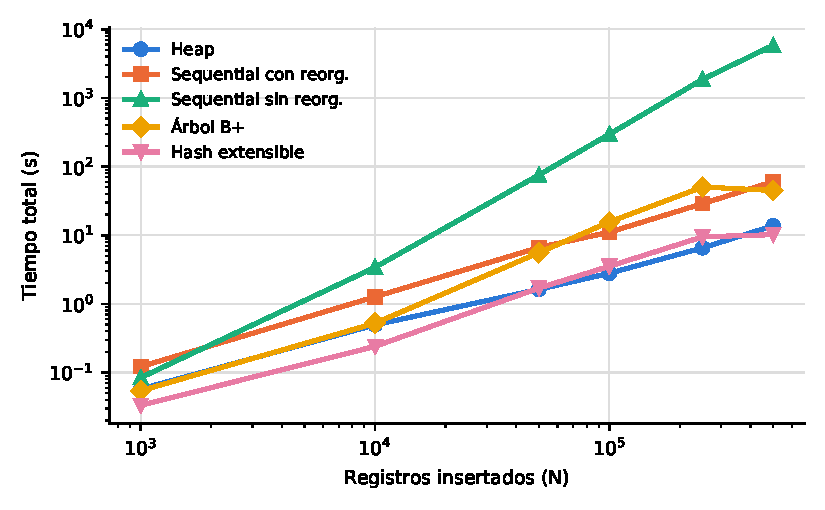
\includegraphics[width=0.8\textwidth]{exp1_tiempo.pdf}
  \caption{Tiempo total de inserción según $N$ (ambos ejes en escala logarítmica).}
\end{figure}

\begin{figure}[H]
  \centering
  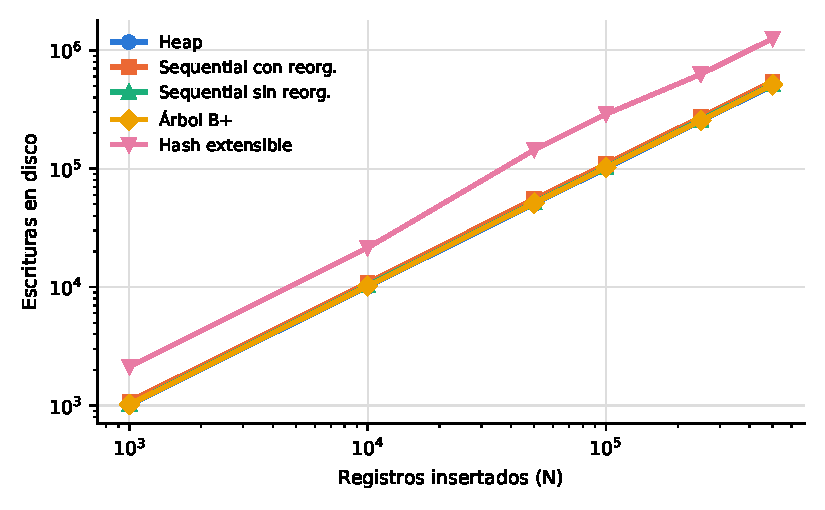
\includegraphics[width=0.8\textwidth]{exp1_escrituras.pdf}
  \caption{Escrituras en disco según $N$ (ambos ejes en escala logarítmica).}
\end{figure}

\begin{center}
\begin{tabular}{lrr}
\toprule
Estructura ($N = 500\,000$) & Tiempo (s) & Escrituras \\
\midrule
Heap & 13,7 & 503\,970 \\
Hash extensible & 10,2 & 1\,255\,355 \\
Árbol B+ & 44,8 & 510\,575 \\
Sequential con reorganización & 60,4 & 546\,409 \\
Sequential sin reorganización & 5\,833,3 & 517\,254 \\
\bottomrule
\end{tabular}
\end{center}

\begin{itemize}
  \item \textbf{Heap} escribe casi exactamente una página por registro: la inserción
        es O(1), como se esperaba.
  \item \textbf{Sequential sin reorganización} crece mucho más rápido que el resto:
        de 3,4 s con $10^4$ a casi 97 minutos con $5\cdot10^5$. Las cadenas de overflow
        se alargan sin límite y cada inserción las recorre enteras.
  \item \textbf{Sequential con reorganización} se mantiene casi lineal. El límite $K$
        hace que las cadenas nunca pasen de $\approx \log_2 P$ páginas; el costo de
        reescribir el archivo se reparte entre las $K$ inserciones que lo provocan.
  \item \textbf{Hash} escribe unas 2,5 veces más que el Heap: cada split reescribe el
        bucket y su hermano, y cada duplicación reescribe el directorio. Aun así es el
        más rápido, porque cada inserción lee solo una entrada del directorio y un
        bucket.
  \item \textbf{B+} escribe cerca de una página por inserción (la hoja), más los
        splits ocasionales. El tiempo es mayor porque cada inserción desciende $h$
        niveles. El valor de $2{,}5\cdot10^5$ (50,4 s) supera al de $5\cdot10^5$
        (44,8 s); lo atribuimos a que los procesos corrían en paralelo y compitieron
        por el disco.
\end{itemize}

\subsection{Experimento 2: búsquedas de igualdad}

\begin{figure}[H]
  \centering
  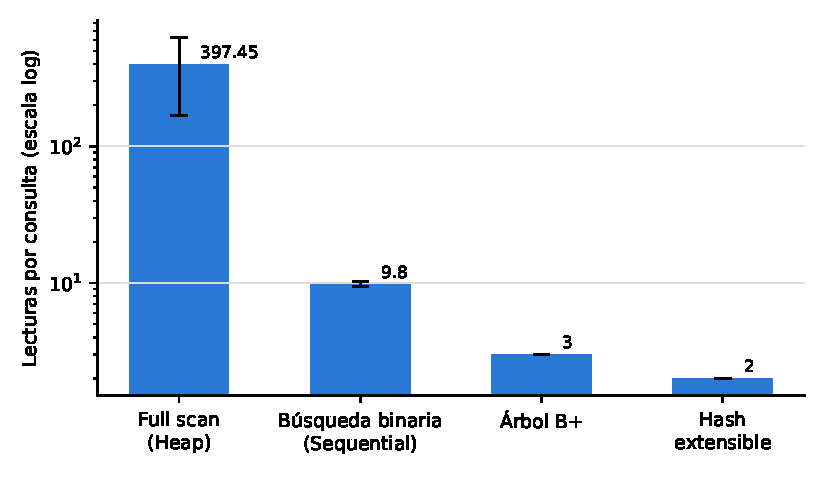
\includegraphics[width=0.75\textwidth]{exp2_lecturas.pdf}
  \caption{Lecturas por consulta: media y desviación estándar (escala logarítmica).}
\end{figure}

\begin{figure}[H]
  \centering
  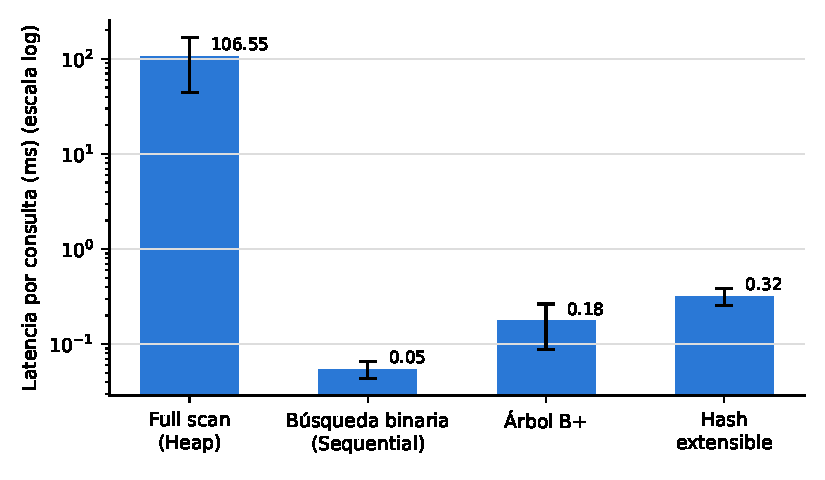
\includegraphics[width=0.75\textwidth]{exp2_latencia.pdf}
  \caption{Latencia por consulta: media y desviación estándar (escala logarítmica).}
\end{figure}

\begin{center}
\begin{tabular}{lrrrr}
\toprule
Acceso & Lecturas & Desv. & Latencia (ms) & Desv. \\
\midrule
Full scan (Heap) & 397,5 & 228,8 & 106,55 & 61,97 \\
Búsqueda binaria (Sequential) & 9,8 & 0,4 & 0,05 & 0,01 \\
Árbol B+ & 3 & 0 & 0,18 & 0,09 \\
Hash extensible & 2 & 0 & 0,32 & 0,07 \\
\bottomrule
\end{tabular}
\end{center}

\begin{itemize}
  \item \textbf{Full scan:} el Heap tiene $P = 794$ páginas. La búsqueda se detiene al
        encontrar la clave, así que en promedio lee $P/2 \approx 397$. La desviación
        es alta porque depende de dónde cayó la fila.
  \item \textbf{Búsqueda binaria:} $\approx \lceil \log_2 P \rceil$ lecturas, con
        desviación casi nula.
  \item \textbf{B+:} siempre 3 lecturas, igual a la altura del árbol. Desviación 0.
  \item \textbf{Hash:} siempre 2 lecturas: una página del directorio y el bucket.
  \item En latencia, la búsqueda binaria es la más rápida pese a leer más páginas:
        su código es más simple que el descenso del B+ o la lectura de entradas del
        Hash. Con un disco real y sin caché del sistema operativo, el orden seguiría
        al de las lecturas.
\end{itemize}

\subsection{Experimento 3: rangos con selectividad variable}

\begin{figure}[H]
  \centering
  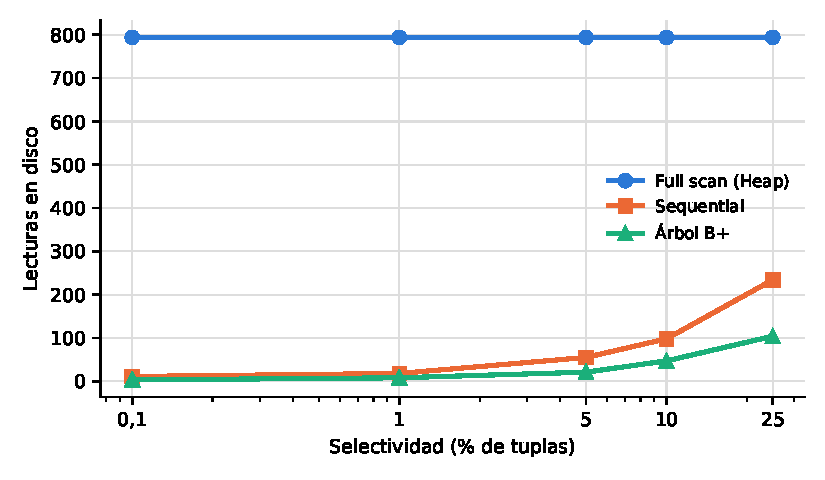
\includegraphics[width=0.75\textwidth]{exp3_lecturas.pdf}
  \caption{Lecturas en disco según la selectividad del rango.}
\end{figure}

\begin{figure}[H]
  \centering
  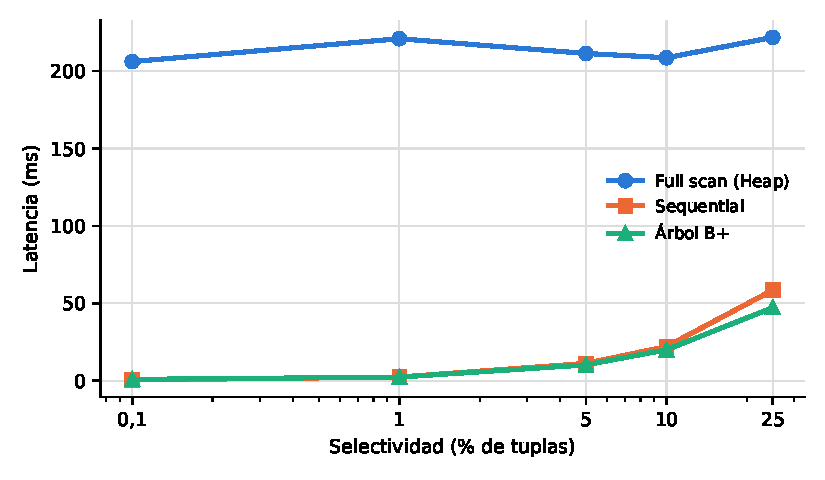
\includegraphics[width=0.75\textwidth]{exp3_latencia.pdf}
  \caption{Latencia según la selectividad del rango.}
\end{figure}

\begin{center}
\begin{tabular}{lrrr}
\toprule
Selectividad & Full scan (Heap) & Sequential & Árbol B+ \\
\midrule
0,1\,\% & 794 & 11 & 3 \\
1\,\% & 794 & 18 & 8 \\
5\,\% & 794 & 55 & 21 \\
10\,\% & 794 & 98 & 47 \\
25\,\% & 794 & 234 & 104 \\
\bottomrule
\end{tabular}
\end{center}

\begin{itemize}
  \item \textbf{Full scan} es constante: siempre lee las 794 páginas, sin importar
        cuántas filas devuelve.
  \item \textbf{Sequential} paga la búsqueda binaria ($\approx 10$ lecturas) y luego
        recorre en orden las páginas del rango.
  \item \textbf{B+} paga el descenso (3 lecturas) y luego recorre hojas. Sus hojas
        guardan entradas de 12 bytes en vez de filas de 32, así que caben más por
        página y lee menos de la mitad que el Sequential.
  \item Ambos crecen en forma lineal con la selectividad. Con 25\,\% todavía están muy
        por debajo del full scan; el punto de cruce estaría por encima de esa
        selectividad.
\end{itemize}

\subsection{Experimento 4: tamaño de bloque}

\begin{figure}[H]
  \centering
  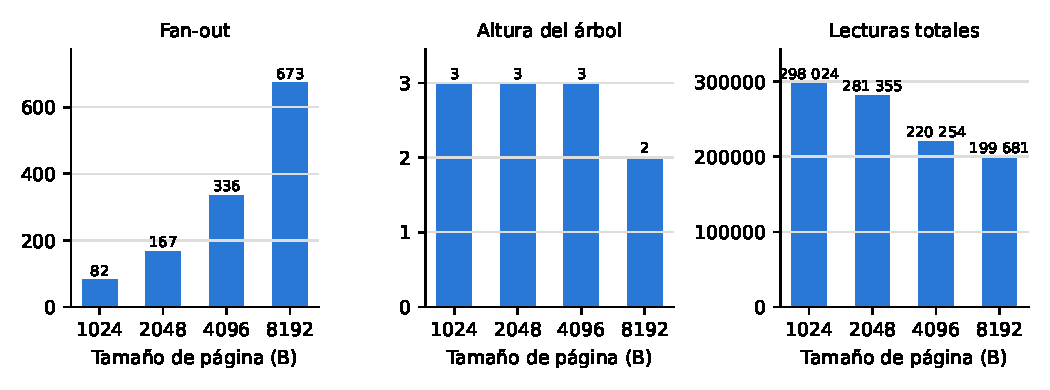
\includegraphics[width=\textwidth]{exp4_bloque.pdf}
  \caption{Fan-out, altura y lecturas totales del B+ según el tamaño de página.}
\end{figure}

\begin{center}
\begin{tabular}{rrrrr}
\toprule
$B$ (bytes) & Fan-out & Altura & Lecturas & Escrituras \\
\midrule
1024 & 82 & 3 & 298\,024 & 108\,887 \\
2048 & 167 & 3 & 281\,355 & 104\,476 \\
4096 & 336 & 3 & 220\,254 & 102\,329 \\
8192 & 673 & 2 & 199\,681 & 101\,226 \\
\bottomrule
\end{tabular}
\end{center}

\begin{itemize}
  \item El fan-out se duplica cada vez que se duplica $B$, porque la capacidad de un
        nodo es proporcional al tamaño de página.
  \item La altura sigue $h = \lceil \log_M N \rceil$: con $N = 100\,000$ y $M = 673$
        basta con 2 niveles; con $M \le 336$ hacen falta 3.
  \item Las lecturas bajan al crecer $B$: nodos más anchos significan menos splits y,
        con 8 KB, un nivel menos que recorrer en cada inserción.
  \item Las escrituras bajan poco (de 108\,887 a 101\,226): casi todas son la
        escritura de la hoja en cada inserción, que no depende de $B$.
\end{itemize}

\section{Conclusiones}

\begin{itemize}
  \item Contar I/O en el único punto que toca el disco (el Pager) hizo que los
        resultados coincidan con las fórmulas de costo: $P/2$ para el full scan,
        $\log_2 P$ para la búsqueda binaria, $h$ para el B+ y 2 para el Hash.
  \item Para igualdades, el Hash extensible es el acceso más barato en lecturas. Para
        rangos, el B+ es el mejor: lee menos que el Sequential File porque sus hojas son
        más compactas que las filas.
  \item El Sequential File sin reorganización no escala. El límite $K$ derivado del
        costo de búsqueda lo mantiene en tiempo casi lineal.
  \item Páginas más grandes aumentan el fan-out y reducen la altura del B+, lo que
        baja el total de lecturas.
\end{itemize}

\end{document}
